\documentclass[oneside,spanish]{amsart}
\usepackage[T1]{fontenc} % Tipo de fuente
\usepackage[utf8]{inputenc} % Archivo UTF-8
\usepackage[a4paper]{geometry}
\geometry{verbose,tmargin=2cm,bmargin=2cm,lmargin=3cm,rmargin=2.5cm} % Tamaño
\usepackage{amsthm} 
%\usepackage{amsaddr} % Para modificar la posición de address
\usepackage[spanish]{babel} % Idioma español
\usepackage[backend=biber,style=alphabetic,natbib,maxalphanames=1]{biblatex} % Compilar bibliografía con BibLaTeX (no BibTeX)
\usepackage[shortlabels]{enumitem} % Mejora el entorno enumerate
\usepackage{graphicx} % Colocar imágenes
\usepackage[hidelinks]{hyperref} % Vínculos y referencias interactivas
\usepackage[skip=3pt]{caption} % Permite modificar el espacio entre el caption y la imagen
\usepackage{multicol} % Entornos de múltiples columnas
\usepackage{tcolorbox}
\usepackage{listings}

\lstset{basicstyle=\scriptsize\ttfamily,breaklines=true,tabsize=3,
	literate=%
	{ñ}{{\~n}}1
	{Ñ}{{\~N}}1
	{á}{{\'a}}1
	{é}{{\'e}}1
	{í}{{\'i}}1
	{ó}{{\'o}}1
	{ú}{{\'u}}1
	{Á}{{\'A}}1
	{É}{{\'E}}1
	{Í}{{\'I}}1
	{Ó}{{\'O}}1
	{Ú}{{\'U}}1
}

%-------------------------------------------------------------------------
% Configuraciones iniciales
\makeatletter
%Numeración
\numberwithin{equation}{section}
\newlength{\lyxlabelwidth}      % Longitud auxiliar
\makeatother
%-------------------------------------------------------------------------

%-------------------------------------------------------------------------
% Bibliografía
\defbibheading{bibliography}[\refname]{}
\addbibresource{refs-com02.bib}

\renewcommand*{\labelalphaothers}{}

\DeclareLabelalphaTemplate{
	\labelelement{
		\field[final]{shorthand}
		\field{labelname}
		\field{label}
	}
	\labelelement{
		\literal{,\addhighpenspace}
	}
	\labelelement{
		\field{year}
	}
}
%-------------------------------------------------------------------------

%-------------------------------------------------------------------------
% Otras configuraciones
%\pagestyle{plain} % Para que el encabezado esté vacío
\addto\captionsspanish{\renewcommand{\tablename}{Tabla}}
\addto\captionsspanish{\renewcommand{\figurename}{Figura}}

\theoremstyle{definition}
\newtheorem{actividad}{Actividad}
\newtheorem{propuesta}{\bfseries Propuesta}
%-------------------------------------------------------------------------

\usepackage{fancyhdr}
\pagestyle{fancy}
\fancyhf{} % sets both header and footer to nothing
\renewcommand{\headrulewidth}{0pt}
\fancyhead[C]{\scriptsize\MakeUppercase\shorttitle}

%-------------------------------------------------------------------------

% Y acá comienza el documento

\begin{document}
	
%-------------------------------------------------------------------------
% Datos del artículo
\title[Una propuesta de enseñanza de temas relativos a test de hipótesis con el uso de dispositivos móviles]{Una propuesta de enseñanza de temas relativos a test de hipótesis con el uso de dispositivos móviles\vspace{-2ex}}
\author[1]{María Valeria Calandra\textsuperscript{1}}
\address[1,3,4]{UIDET GAMEFI, Dto. Ciencias Básicas, Facultad de Ingeniería, Universidad Nacional de La Plata}
\author[2]{Paula D'Urzo\textsuperscript{2}}
\address[2]{Dto. Ciencias Básicas, Facultad de Ingeniería, Universidad Nacional de La Plata}
\author[3]{Anyelen Di Paolantonio\textsuperscript{3}}
\author[4]{Cecilia De Cortazar\textsuperscript{4}}
\email[corresponding author]{\textsuperscript{1}mava\_calandra@hotmail.com}
%-------------------------------------------------------------------------

\begin{abstract}
	En el marco de la búsqueda de herramientas educativas para la mejora de la enseñanza de la matemática, y en particular de probabilidades y estadística, se presenta una propuesta de trabajo orientada a buscar una alternativa para la enseñanza de temas relativos a test de hipótesis en estadística. La misma serviría para resignificar diversos temas específicos dentro de esta temática mediante la aplicación de inferencia informal con el uso de la aplicación para dispositivos móviles y web. Se realiza además una exploración bibliográfica sobre las dificultades que en la enseñanza y aprendizaje de estos conceptos.    
\end{abstract}

\maketitle
\thispagestyle{empty}

\section{Introducción}

Los métodos de inferencia estadísticos son de fundamental importancia en toda situación que requiera el análisis de datos para la toma de decisiones en presencia de incertidumbre y variación. Contribuye a facilitar el análisis de información que se requiera, (\citet{vanderman02}). \citet{viles07} comenta que la estadística es importante en la ciencia en general, se puede aplicar al diseño de nuevos productos y a su desarrollo, así como al control, a la optimización y a la mejora de la calidad de procesos de fabricación de bienes y servicios.

El objetivo de este trabajo es desarrollar dispositivos que promuevan la enseñanza funcional de esos temas específicos de test de hipótesis para los alumnos de carreras científico-tecnológicas.  Según \citet{batanero17} cuando los alumnos universitarios se encuentran en un curso inicial de estadística y deben resolver un contraste de hipótesis, con frecuencia no comprenden todos los pasos, sino que los aplican en forma mecánica.

Dentro de los temas más importante de inferencia estadística para la aplicación en el campo de experimental, se encuentra el tema de test de hipótesis, pero también son abundantes los reportes sobre las dificultades sobre su enseñanza y aprendizaje. Los cálculos e interpretación de los errores de Tipo I y de Tipo II son fundamentales para entender la lógica de los test de hipótesis. Por eso es que se propone una enseñanza contextualizada, para estas temáticas con el uso de una aplicación que se puede implementar en código de programación R (\citet{teamrc21}) en teléfonos móviles en el que los alumnos pueden simular el proceso de extracción de una muestra aleatoria de una fábrica bajo ciertas condiciones para realizar la certificación de un artículo mediante un test de hipótesis y calcular empíricamente las probabilidades de errores de Tipo I y de Tipo II. El estudiante tiene a su disposición el código del programa y lo puede modificar de modo de simular distintos escenarios de trabajo. Esta propuesta permitiría emular el trabajo científico de investigación en inferencia estadística que parte de un hecho empírico para luego generalizarlo a la población.  Además, los acerca a manejar el lenguaje de programación R de fundamental importancia en el trabajo científico en el campo de la estadística. Esta propuesta permitiría que los alumnos tomen un rol activo en la construcción del conocimiento de estas temáticas ya que pueden intervenir desde la simulación de la muestra con la que se realizará el test como en la construcción de común acuerdo en el transcurso de la clase de los conceptos de error de Tipo I y de Tipo II y la resignificación de los mismos para la situación planteada.

\section{Requisitos previos}

Esta propuesta está dirigida a docentes de nivel superior para la enseñanza en carreras científico-tecnológicas.

\section{Desarrollo}

\subsection{Estado y situación del tema}

Una prueba de hipótesis es un método de inferencia estadístico que permite decidir acerca del valor de un parámetro poblacional por medio de los datos obtenidos a partir de una muestra. Dado el carácter aleatorio de la muestra los resultados pueden estar sujetos a variaciones aleatorias, por lo que una prueba de hipótesis permite decidir si pequeñas desviaciones observadas respecto al resultado que idealmente debería haber ocurrido según nuestra hipótesis, son atribuibles al azar o efectivamente los resultados no se corresponden con la hipótesis que se ha planteado sobre el valor del parámetro. Existen numerosos errores e interpretaciones incorrectas del contraste de hipótesis, que se han encontrado incluso en los trabajos de investigación (\citet{batanero00}; \citet{falk95}; \citet{harradine11}).El establecimiento de hipótesis adecuadas a la situación es el primer paso en la resolución de un problema de contraste de hipótesis pero presenta grandes dificultades de comprensión para los estudiantes que no logran identificar cuáles serían las hipótesis adecuadas en cada caso, no comprenden el papel que juegan en el proceso o confunden las hipótesis nula y alternativa (\citet{vallecillos97}). \citet{liu09} encontraron una falta de comprensión de la lógica de los test de hipótesis ligada a la comprensión de los resultados. Además, \citet{vallecillos94} realizó una amplia investigación sobre el aprendizaje del tema del contraste de hipótesis estadísticas en alumnos universitarios y detectó que algunos alumnos suponen que la suma de las probabilidades de cometer un error de Tipo I y un error de Tipo II es uno y esto no es así, los dos tipos de errores son eventos incompatibles, pero no son sucesos complementarios.  Se han encontrado estudiantes que creen que el cambio del nivel de significación no afecta al riesgo de error de Tipo I en la decisión. Algunos confunden la significación estadística y con relevancia práctica, otros asocian un resultado significativo como uno que corrobora la hipótesis nula. \citet{batanero17} observó que los alumnos manifiestan una dificultad en cuanto a la comprensión, cuando calculan la probabilidad de cometer un error de Tipo I perdiendo de vista la condición (la verdad de la hipótesis nula). Muchos estudiantes asocian de forma inmediata el rechazo de la hipótesis al error de Tipo I. \citet{vallecillos97} encontró conflictos en la lógica de la interpretación de los test de hipótesis ligadas a la suposición de que los test de hipótesis proporcionan una demostración matemática deductiva de la verdad de la hipótesis y que el nivel de significación de un test es la probabilidad de que $H_0$ sea cierta dado que se ha rechazado. Es decir, se interpreta incorrectamente el resultado del test por creer que el contraste demuestra la hipótesis o porque calcula su probabilidad. También en la misma publicación se identifican errores en el aprendizaje de los alumnos asociados al cálculo e interpretación del $p$-valor. El valor $p$ se calcula mediante el cálculo de la probabilidad de observar el valor empírico del estadístico o un valor más extremo, dado que la hipótesis nula es verdadera y varía de una muestra a otra y muchas veces es confundido con el nivel de significación que fija el experimentador antes de realizar el test.  Un concepto que se suele comprender erróneamente es el nivel de significación. Respecto a este concepto se pueden encontrar numerosos conflictos, el más frecuente consiste en intercambiar los dos términos de la probabilidad condicional, interpretándolo como la probabilidad de que la hipótesis nula sea cierta, una vez que la decisión de rechazarla se ha tomado (\citet{krauss02}). También se han reportado conflictos para distinguir lo que es un parámetro y lo que es un estadístico o no reconocen que un estadístico es una variable aleatoria, lo que lleva a plantear mal los test de hipótesis, por ejemplo, los alumnos confunden la media muestral con la media poblacional (\citet{korin21}; \citet{harradine11}).

\subsection{Marco teórico}

Las nuevas teorías didácticas conciben al alumno como un verdadero protagonista de su aprendizaje, en donde el profesor proponga actividades contextualizadas dentro de su especialidad que permitan el surgimiento de un modo funcional las técnicas, elementos tecnológicos y organizaciones matemáticas que se quieren enseñar. Los docentes deben ser guías y mediadores, para que los estudiantes aprendan. La Teoría Antropológica de lo Didáctico (TAD), propone la aplicación de un dispositivo didáctico que denomina Actividad de Estudio e Investigación (AEI), para enfrentar lo que ha denominado la monumentalización del saber y la pérdida del sentido de lo que se estudia en algunos ámbitos educativos (\citet{chevallard13}). Dicho dispositivo permite introducir en los sistemas de enseñanza procesos de estudio funcionales, tanto a nivel cognitivo como procedimental, concibiendo al alumno con un rol activo en el proceso de enseñanza/aprendizaje Para ello, las AEI se organizan en torno a una pregunta generatriz $Q_0$, seleccionada por el profesor, que tenga el potencial de generar el estudio por parte de los alumnos de ciertos contenidos matemáticos. Se propone una investigación y debate, en este caso, centrado en torno a la pregunta generatriz: $Q_0$: \textit{¿Cómo certificar una característica de un producto o proceso?}. La búsqueda de respuesta a la pregunta también generará más preguntas derivadas, que permitirán contextualizar la propuesta, como puede ser ¿Cómo certificar la longitud del alabe de la turbina de un motor? Las respuestas a las preguntas junto con otras derivadas de una actividad específica llevarán al estudio de técnicas y de elementos tecnológicos-teóricos específicos relativos a test de hipótesis.

\subsection{Propuesta}

La propuesta que se presenta a continuación está dirigida, en particular, a alumnos de las carreras científico-tecnológicas que estén cursando probabilidades y estadística. La AEI servirá para complementar la enseñanza formal de estos conceptos y se resolverá  mediante la aplicación de inferencia informal (\citet{zieffler08}) con  el uso de la aplicación para dispositivos móviles y web: Run R Script - Online Statistical Data Analysis - Version 1.1 (\cite{liila18}) que permite programar usando el lenguaje R versión 3.5.2 (\cite{teamrc21}), y Python (\cite{python17}), es un entorno de desarrollo integrado (IDE) en línea, incluye una consola, un editor de código que admite la ejecución directa de código, así como herramientas, archivos de datos definidos por el usuario, almacenamiento de código en la nube. Este software genera una cuenta en la nube para cada usuario, donde se almacenan los códigos que desee el mismo, con el fin de ser compartidos con los usuarios mediante diferentes métodos (redes sociales, email, etc.), permitiendo ser ejecutados sin poseer una instalación del programa. Se propone, en este caso, compartir con los alumnos en el aula las rutinas mediante un código QR que “encripte” el link a la dirección web de la rutina en forma directa. 

Para comenzar la actividad el profesor propone un debate acerca de la certificación de un producto y de los métodos estadísticos para certificar la calidad del mismo, que iniciará el estudio del saber a construir. La pregunta generatriz del debate será: $Q_0$: \textit{¿Cómo certificar una característica de un producto?}, esta pregunta actuaría como eje articulador para la reconstrucción de los temas relativos a test de hipótesis. A su vez esta pregunta podría derivar en otras \textit{¿Qué significa certificar un producto?} La certificación de un producto o proceso consiste en un gran número de actividades tendientes a validar la calidad del mismo, dichas actividades dependerán del producto a certificar. Consiste en la inspección de los procesos de fabricación, ensayos de muestras realizadas por el organismo de certificación correspondiente y la auditoría de las mismas para verificar si cumplen los estándares técnicos. \textit{¿Qué productos se pueden certificar?} Materiales de construcción de distinta índole, partes de aeronaves, materiales eléctricos, productos electrónicos, etc. \textit{¿Qué característica de un producto se podría certificar?}

Supongamos el caso en que se desea certificar una dimensión de un alabe de turbina de un motor a reacción de un avión (ver Figura \ref{fig:1}).

\begin{figure}[h]
	\centering
	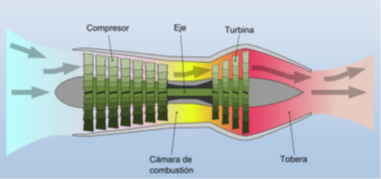
\includegraphics[height=0.3\linewidth]{Anexos-06/Imagen1}
	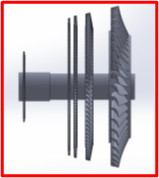
\includegraphics[height=0.3\linewidth]{Anexos-06/Imagen2}
	\caption{Esquema típico de un motor a reacción de avión, a la izquierda el rotor de la turbina de varios discos}
	\label{fig:1}
\end{figure}

Como se observa en la sección de la turbina existen varios discos conformados por una cierta cantidad de alabes, insertados en los mismos, estos deben poseer una longitud media específica en función del diseño del motor (Ver Figura \ref{fig:2}).

\begin{figure}[h]
	\centering
	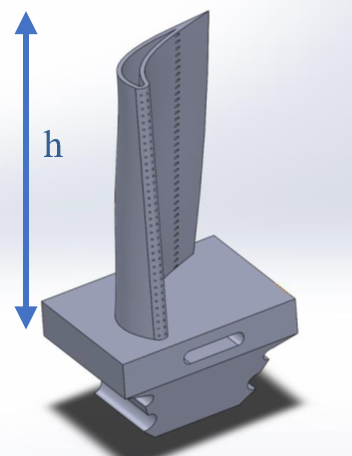
\includegraphics[height=0.3\linewidth]{Anexos-06/Imagen3}
	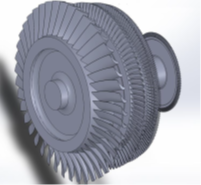
\includegraphics[height=0.3\linewidth]{Anexos-06/Imagen4}
	\caption{Imagen de un alabe y de los discos donde se insertan los mismos}
	\label{fig:2}
\end{figure}

En un caso particular, de un motor de una marca determinada, la longitud de un alabe para el disco de mayor diámetro se puede modelar como una variable aleatoria con distribución aproximadamente Normal con media $\mu= 269$ mm, y una desviación estándar $\sigma = 0.15$ mm.

\begin{tcolorbox}[arc=0mm,colback=white]
	\begin{actividad}
		Una fábrica de motores a reacción está trabajando de acuerdo a los estándares de calidad. De todas formas, anualmente debe someterse a una auditoría para verificar dicha situación. La auditoría se realiza mediante un test de hipótesis realizado sobre una muestra aleatoria extraída de la producción. La característica a certificar es la longitud media del álabe para el disco de mayor diámetro
	\end{actividad}
\end{tcolorbox}

\begin{propuesta}\label{prop:1}
	El objetivo de esta propuesta es resignificar desde un punto de vista empírico el concepto de error de Tipo I y de probabilidad de error de Tipo I para un test de hipótesis.
\end{propuesta}

Para realizar la actividad se le propone a cada alumno generar con la aplicación Run R Script una muestra aleatoria $X_1, X_2, ..., X_10$ donde cada $X_i$ tenga distribución Normal con media 269 y desviación estándar $\sigma = 0.15$ mm, que serviría para simular la extracción de una muestra aleatoria de la fábrica que está trabajando de acuerdo a los estándares de calidad. 

Para poder realizar la certificación de la longitud media de la producción de los álabes de esa marca producidos por una fábrica, se propone a cada alumno, realizar con la muestra obtenida el siguiente test de hipótesis bilateral:

$H_0: \mu =269$ mm, contra la hipótesis alternativa $H_1: \mu \ne 269$ mm

Donde rechazar $H_0$ significaría que la fábrica no cumple los estándares. La regla de decisión del test podría ser rechazar $H_0$ si $\biggl|\frac{\bar{X} - 269}{\bigl(\frac{0.15}{\sqrt{10}}\bigr)}\biggr| > z_{0.05}$ siendo $\bar{X} = \frac{X_1 + X_2 + ... + X_{10}}{10}$.

Luego se plantea a los estudiantes las siguientes preguntas \textit{¿Alguno rechazó $H_0$ con la muestra seleccionada? ¿Es correcto haber rechazado $H_0$? ¿Si se realiza el test 10.000 veces con distintas muestras, cuantas veces rechazaríamos $H_0$? ¿Se podría representar gráficamente usando las 10.000 muestras de tamaño 5 la distribución empírica de $\bar{X}$? ¿Cómo se podría representar la región de rechazo de $H_0$ en dicha gráfica?  ¿Cómo se podría calcular la frecuencia relativa de veces que la fábrica no satisface los estándares de calidad? ¿Cómo se podría interpretar esa proporción en términos de nuestro problema? ¿Cómo se podría calcular la frecuencia relativa de veces que la fábrica podría certificar la pieza?}

Para contestar estas preguntas los estudiantes pueden correr una rutina utilizando Run R Script con el código que se muestra a continuación que se brinda a los mismos mediante la vinculación con un código QR \url{https://r.varisk.xyz/r/220611/demo-Rout-1558816771-dark.html}

\begin{lstlisting}
	n=10
	mediaMuestral=function(n)   #Esta función genera una muestra aleatoria de tamaño n 
	{muestra=rnorm(n,269,0.15) # Normal con media 269 y desviación estándar 0,15
		media=mean(muestra)            # calcula la media de dicha muestra
		return(media)}
	mediaMuestral(5)                   # el programa muestra la media obtenida
	muchasmedias=replicate(10000,mediaMuestral(5))  # se generan 10000 medias muestrales                                                                       
	z=qnorm(0.05,lower.tail=FALSE)            # calcula el z0.05             
	hx=hist(muchasmedias,breaks=50)          # se genera el histograma.
	plot(hx,col=ifelse(abs(hx$breaks-269)< z*0.15/sqrt(5),0,3))  # colorea la region de rechazo
	porc=1-sum(abs(muchasmedias-269)<e)/10000   # estima la probabilidad de error de tipo I
\end{lstlisting}

\begin{figure}[h]
	\centering
	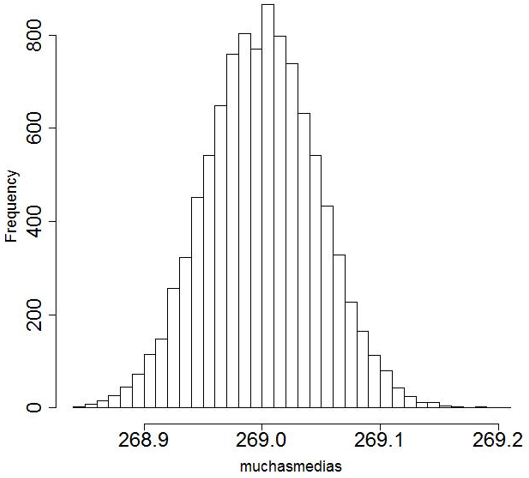
\includegraphics[height=0.4\linewidth]{Anexos-06/Imagen5}
	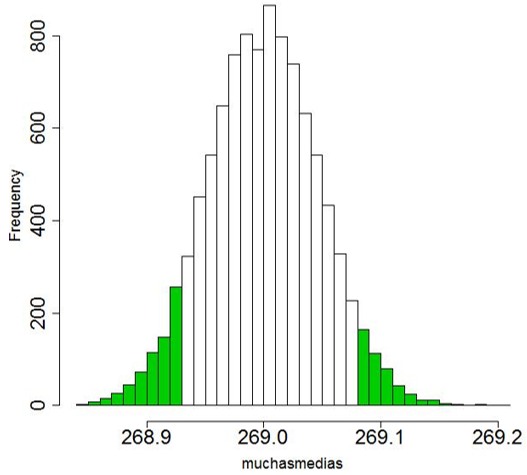
\includegraphics[height=0.4\linewidth]{Anexos-06/Imagen6}
	\caption{Histogramas de la distribución de frecuencias de las medias muestrales Propuesta \ref{prop:1}}
	\label{fig:3}
\end{figure}

El saber hacer estas tareas se justifica por el hecho de cada alumno puede generar sus propias muestras e identificar gráficamente la distribución de las frecuencias absolutas de $\bar{X}$ cuando la distribución subyacente de la muestra es Normal con media 269 y desviación estándar $0.15$ (Figura \ref{fig:3}, izquierda). Esto serviría para contestar la pregunta: ¿Se podría representar gráficamente usando las 10.000 muestras de tamaño 5 la distribución empírica de $\bar{X}$? Luego pueden identificar gráficamente en color verde en el histograma (Figura \ref{fig:3}, derecha), la frecuencia de veces que se rechazará $H_0$ con lo que se puede estimar la probabilidad de cometer un error de Tipo I si se la divide por 10.000:
\begin{equation*}
	P(\text{error de Tipo I}) = P(\text{Rechazar $H_0$}|\mu=269) \cong \frac{103}{10000}
\end{equation*}

Esta, difiere un poco de la verdadera probabilidad que es $0,1$ por tratarse de una simulación.

Esto serviría para contestar estas preguntas: \textit{¿Qué proporción de $\bar{X}$ caen en la zona de rechazo? ¿Cómo se podría interpretar esa proporción en términos de nuestro problema?}

En el mismo gráfico de la Figura \ref{fig:3} de la derecha, se puede apreciar la región complementaría, que no está pintada de verde, que serviría para estimar la potencia o sensibilidad del test.

Esta forma de trabajo les intervenir en el diseño del programa realizando distintas tareas: generar las muestras aleatorias bajo las condiciones requeridas, calcular el promedio de cada una de ellas, construir un histograma con los promedios, identificar en el histograma los promedios que caen en la zona de rechazo del test, cambiar si quisieran el tamaño de las muestras o el número de simulaciones. Por otro lado, esta propuesta permitiría que los alumnos se familiaricen con el uso del lenguaje de programación R, que es fundamental para cálculos en estadística. Esta forma de trabajo muestra cómo se llevan a cabo las investigaciones estadísticas y las principales ideas que subyacen en dichas investigaciones.

\begin{propuesta}\label{prop:2}
	El objetivo de esta propuesta es resignificar desde un punto de vista empírico el concepto de error de Tipo II y de probabilidad de error de Tipo II para el test de hipótesis aplicado a la misma actividad.
\end{propuesta}

Para realizar la actividad se le propone a cada alumno generar con la aplicación Run R Script una muestra aleatoria $X_1,X_2,..., X_{10}$ donde cada $X_i$ tenga distribución Normal con media $269.04$ y desviación estándar $\sigma = 0.15$ mm, que serviría para simular la extracción de una muestra aleatoria de la fábrica que no está trabajando de acuerdo a los estándares de calidad.

Luego se plantean las preguntas \textit{¿Algún alumno no pudo rechazar $H_0$ con la muestra seleccionada? ¿Si se realiza el test 10000 veces con distintas muestras, cuantas no veces rechazaríamos $H_0$? ¿Se podría representar gráficamente usando las 10000 muestras de tamaño 5 la distribución empírica de $\bar{X}$? ¿Para qué proporción de valores de $\bar{X}$ se rechaza $H_0$? ¿Qué proporción de valores de $\bar{X}$ no caen en la zona de rechazo? ¿Cómo se podría identificar esa región en el histograma? ¿Cómo se podría interpretar esta proporción en términos de nuestro problema? ¿Qué proporción de valores de $\bar{X}$ caen en la zona de rechazo de $H_0$? ¿Cómo se podría interpretar esta proporción en términos de nuestro problema?}

Para contestar estas preguntas los estudiantes pueden correr una rutina utilizando Run R Script con el código que se muestra a continuación que se brinda a los mismos mediante la vinculación con un código QR \url{https://r.varisk.xyz/r/220611/demo-Rout-1530181579-dark.html}

\begin{lstlisting}
	mediaMuestral=function(n)	# la función genera una muestra aleatoria de tamaño n de 
	{muestra=rnorm(n,269.04,0.15)	# distribución Normal con media 269,04 y desviación estándar 0,15
		media=mean(muestra)	# calcula la media de dicha muestra
		return(media)}
	mediaMuestral(5)	# el programa muestra la media obtenida
	muchasmedias=replicate(10000,mediaMuestral(5))	# se generan 10000 medias muestrales  
	z=qnorm(0.05,lower.tail=FALSE)		# calcula el z0.05             
	hx=hist(muchasmedias,breaks=50)		# se genera el histograma.
	plot(hx,col=ifelse(abs(hx$breaks-269)< z*0.15/sqrt(5),2,0))	# identifica la zona de aceptación
	porc=sum(abs(muchasmedias-269)<e)/10000		# estima la probabilidad de error de tipo II
\end{lstlisting}

\begin{figure}[h]
	\centering
	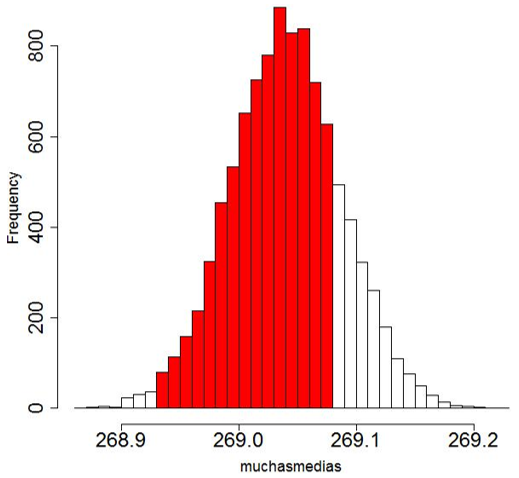
\includegraphics[height=0.4\linewidth]{Anexos-06/Imagen7}
	\caption{Histogramas de la distribución de frecuencias de las medias muestrales Propuesta \ref{prop:2}}
	\label{fig:4}
\end{figure}

El alumno puede generar sus propias muestras e identificar la región de aceptación de $H_0$ (ver zona de color rojo en Figura \ref{fig:4}), mediante la distribución empírica de $\bar{X}$ cuando la distribución subyacente de la muestra es Normal con media $269.04$ y desviación estándar $0.15$. Lo que permitiría estimar empíricamente la probabilidad de cometer un error de Tipo II, es decir:
\begin{equation*}
	P(\text{error de Tipo II}) = P(\text{Aceptar $H_0$}|\mu=269.04) \cong \frac{8.431}{10000}
\end{equation*}

Este valor difiere un poco de la verdadera probabilidad por tratarse de una simulación. Se puede realizar nuevamente la experiencia con una muestra de tamaño $n=20$ o más para ver que a medida que se toman muestras más grandes de la producción dicha probabilidad disminuye. También se podría generar muestras con una media más lejos de 269, por ejemplo $269.06$ en lugar de $269.04$ y observar también que la probabilidad de cometer error de Tipo II disminuye.

\section{Conclusiones}

En este trabajo se presentó una Actividad de Estudio y de Investigación que permitiría resignificar las probabilidades de error de Tipo I y de error de Tipo II, a partir de la simulación de la certificación de una característica de una pieza de un motor. La misma pregunta generatriz es posible presentarla en otros contextos y orientar la propuesta para distintas carreras científico-tecnológicas. El uso de la aplicación Run R Script ofrece grandes ventajas para la enseñanza dado que se puede implementar en un aula de clases, pudiéndose ejecutar en un dispositivo móvil y sin tener la aplicación instalada, esto resulta superador a otras propuestas de este tipo (\citet{batanero15}), ya que esta aplicación no solo tiene esta capacidad, sino que además permite programar y variar los códigos, lo cual expande el universo de posibilidad de estudios de diferentes aspectos de la temática. Además, se les facilita a los estudiantes el código del programa propuesto para la actividad, de modo que ellos simplemente lo ejecuten como está o puedan cambiar algunas variables para explorar el comportamiento de las probabilidades de los errores de Tipo I y II en distintas situaciones, como por ejemplo: ¿Qué pasa con dichas probabilidades si aumentamos el número de piezas extraída de la fábrica? El hecho de usar la simulación para los cálculos los ayudaría a comprender mejor cuál es la función del condicionante en el cálculo de las probabilidades de error de Tipo I y de Tipo II y de sus complementos. Además, permitiría emular el trabajo científico en inferencia estadística que parte de un hecho empírico para luego generalizarlo a la población. Esta propuesta de enseñanza se ha aplicado a alumnos de la facultad de ingeniería de la Universidad Nacional de La Plata, como trabajo futuro se evaluará su impacto en el aprendizaje.

\section{Bibliografía}

\nocite{*}
\printbibliography

\end{document}